\documentclass[letterpaper, 12pt]{article}
\usepackage[top = 1.6cm, left = 2cm, right = 2cm ]{geometry}
\usepackage[pdftex]{graphicx}
\usepackage{soulutf8}
\usepackage{amsmath}
\usepackage{tikz}
\usepackage[utf8]{inputenc}
\usepackage{longtable}
\usepackage[T1]{fontenc}
\usepackage{epigraph}
\usepackage{fancyhdr}
\usepackage{float}
\usepackage{subfig}
\usepackage{xcolor}
\usepackage{eurosym}
\usepackage{calc}
\usepackage{multirow} 
%
%
%%%%% Custom commands
%
%
\def\changemargin#1#2{\list{}{\rightmargin#2\leftmargin#1}\item[]}
\let\endchangemargin=\endlist
%
\newcommand{\newlinealinea}{
~\\ \hspace*{0.5cm}}
%
\newcommand{\alinea}{
\hspace*{0.5cm}}
%
\newcommand{\alinealong}{
\hspace*{1.1cm}}
%
\newcommand{\alignparagraph}{
\hspace*{0.6cm}}
%
\newcommand{\red}[1]{
	\textcolor{red}{#1}}
%
\newcommand{\green}[1]{
	\textcolor{green}{#1}}
%
\newcommand{\point}{$\bullet\ $}
%
\makeatletter
	\newcommand*{\whiten}[1]{\llap{\textcolor{white}{{\the\SOUL@token}}\hspace{#1pt}}}
	\newcommand{\myul}[1]{
		\underline{\smash{#1}}
	}
\makeatother
%
\setlength{\fboxsep}{2pt}
%
\DeclareMathOperator*{\argmax}{\arg\!\max}
%
%
%%%%% Custom text
%
%
\renewcommand*\sfdefault{phv}
\renewcommand*\rmdefault{ppl}
%
\renewcommand\epigraphflush{flushright}
\renewcommand\epigraphsize{\normalsize}
\setlength\epigraphwidth{0.7\textwidth}
%
\definecolor{titlepagecolor}{cmyk}{0.24,0.92,0.78,0.25}
\definecolor{red}{cmyk}{0, 0.91, 0.91, 0.20}
%
\DeclareFixedFont{\titlefont}{T1}{phv}{\seriesdefault}{n}{0.375in}
%
%
%%%%% Header
%
%
\pagestyle{fancy}
\lhead{Anthony Rouneau}
\rhead{MAB1 Sciences Informatiques}
\cfoot{\thepage}
%
%
%%%%% Title page. The following code is borrowed from: 
%%%%%       http://tex.stackexchange.com/a/86310/10898
%
%
\newcommand\titlepagedecoration{%
\begin{tikzpicture}[remember picture,overlay,shorten >= -10pt]

\coordinate (aux1) at ([yshift=-70pt]current page.north east);
\coordinate (aux2) at ([yshift=-460pt]current page.north east);
\coordinate (aux3) at ([xshift=-6cm]current page.north east);
\coordinate (aux4) at ([yshift=-150pt]current page.north east);

\begin{scope}[titlepagecolor!40,line width=12pt,rounded corners=12pt]
\draw
  (aux1) -- coordinate (a)
  ++(225:5) --
  ++(-45:5.1) coordinate (b);
\draw[shorten <= -10pt]
  (aux3) --
  (a) --
  (aux1);
\draw[opacity=0.6,titlepagecolor,shorten <= -10pt]
  (b) --
  ++(225:2.2) --
  ++(-45:2.2);
\end{scope}
\draw[titlepagecolor,line width=8pt,rounded corners=8pt,shorten <= -10pt]
  (aux4) --
  ++(225:0.8) --
  ++(-45:0.8);
\begin{scope}[titlepagecolor!70,line width=6pt,rounded corners=8pt]
\draw[shorten <= -10pt]
  (aux2) --
  ++(225:3) coordinate[pos=0.45] (c) --
  ++(-45:3.1);
\draw
  (aux2) --
  (c) --
  ++(135:2.5) --
  ++(45:2.5) --
  ++(-45:2.5) coordinate[pos=0.3] (d);   
\draw 
  (d) -- +(45:1);
\end{scope}
\end{tikzpicture}%
}
%
\begin{document}
	\begin{titlepage}
	%
	\noindent
	%
	\newgeometry{bottom = 2cm, top = 2.5cm}
	\begin{center}
		
\includegraphics[scale=1.2]{Images/UMONS}\\
			\vspace*{0.3cm}
		
\includegraphics[scale=0.23]{Images/FS_Logo}\\
			\vspace*{2.5cm}
		%
		\titlefont Résumé de Datamining et Datawarehousing \par
		%
	\end{center}
	\vspace*{3cm}
	\hfill
	%
	\begin{minipage}{0.18\linewidth}
		\begin{flushright}
			\rule{0.5pt}{50pt}
		\end{flushright}
	\end{minipage}
	%
	\begin{minipage}{0.8\linewidth}
		\begin{flushleft}
			\textsf{\textbf{Résumé realisé par:}} Anthony Rouneau\\
			\textsf{\textbf{Section:}} 1$^{er}$ Bloc Master en 
				Sciences Informatiques
		\end{flushleft}
	\end{minipage}
	%
	\vspace*{\fill}                                                             
	%
	\begin{center}
		Faculté des Sciences $\bullet$ Université de Mons $\bullet$ 
		Place du Parc 20 $\bullet$ B-7000 Mons
	\end{center}
	%
	\titlepagedecoration
	%
\end{titlepage}
%
%
%%%% Tables des matières
%
%
\newgeometry{top = 3cm, left = 2cm, right = 2cm, bottom=2.5cm}
%
\tableofcontents
%
\newpage
%
%
\part{Classification}
	\section{Introduction}
		\alinea Le but d'une classification est d'assigner des objets
			(instances) à
			une classe selon une suite d'attributs. Chaque objet peut donc
			être représenté par un tuple $(x, y)$, où $x$ est une séquence
			d'attributs et $y$ le nom de sa classe.\\
		%
		\alinea Un \myul{\textbf{attribut}} peut être discret ou continu,
			contrairement au \myul{\textbf{label de classe}}, 
			qui lui doit être discret. Ce qui
			veut dire que le nombre de classes dans lesquelles les instances
			seront classé est fini, et que toutes les classes sont à priori
			connues. \hl{C'est ce qui différencie une classification d'une 
			régression}\\
		%
		~\\
		%
		\myul{\textbf{Classification}}-- \red{Tâche de construire/%
			d'apprendre une fonction $f$ qui fera correspondre un ensemble
			d'attributs, un objet, $x$ à une des classes prédéfinies, $y$.}
		%
		\paragraph{\point Buts d'une classification}~\\~\\
		%
		\begin{tabular}{lp{11cm}}
		    \myul{\textbf{Modélisation descriptive}}& 
		    	\red{Utilisation d'une classification dans le but de lister les
				attributs qui définissent une certaine classe.}
				(e.g. attributs d'animaux $\rightarrow$ famille d'animaux.\\
		    \myul{\textbf{Modélisation prédictive}}&
				\red{Utilisation d'une classification pour prédire la classe
				d'objets inconnus.} Notons qu'une classification n'est pas
				performante pour des classes ordonnées (avec une hiérarchie
				ou un ordre définie).
		\end{tabular}				
		%
	%
	\section{Approche générale}
		\alinea Une technique de classification consiste à construire un
			\myul{modèle} de classification depuis un 
			\myul{\textbf{ensemble de données d'entraînement}}. Ce modèle
			peut ensuite être évalué en y faisant passer un 
			\myul{\textbf{ensemble de données de test}}, idéalement 
			\hl{différent de l'ensemble d'entraînement pour éviter 
			l'\textit{overfiting}} (voir plus loin).\\
		%
		\alinea Un modèle est évalué selon plusieurs métriques,
			dont par exemple la \textit{Précision} et le 
			\textit{Taux d'erreur}.
			\begin{figure}[H]
				\centering
				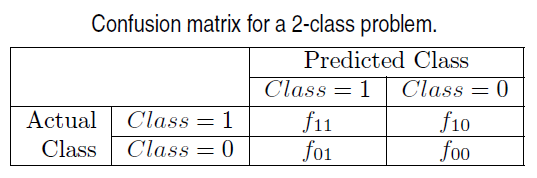
\includegraphics[scale=0.75]{Images/conf_matrix.png}
			\end{figure}\noindent
			\begin{align*}
			\text{Précision} &=& 
			\frac{\text{Nombre de prédictions correctes}}%
			{\text{Nombre total de prédiction}} &=& \frac{f_{11} + f_{00}}%
			{f_{11} + f_{10} + f_{01} + f_{00}}\\
			%			
			\text{Taux d'erreur} &=& 
			\frac{\text{Nombre de prédictions fausses}}%
			{\text{Nombre total de prédiction}} &=& \frac{f_{10} + f_{01}}%
			{f_{11} + f_{10} + f_{01} + f_{00}}\\
			\end{align*}%
		%
	%
	\section{Arbre de décision (DTI)}
		\begin{center}DTI = Decision Tree Induction.\end{center}
		\alinea Le nombre d'arbres de décision pouvant découler d'un ensemble
			d'attributs est exponentiel. Il est donc impossible de trouver
			l'arbre optimal pour un problème de classification donné.
			C'est pourquoi \hl{la plupart des techniques de construction 
			utilisent un algorithme glouton (greedy)}.
		%
		\subsection{Algorithme de Hunt}
			\alinea Les méthodes de construction \texttt{ID3}, \texttt{C4.5},
				\texttt{CART} découlent
				toutes du même algorithme : l'algorithme de Hunt. 
				L'algorithme consiste à partitionner récursivement 
				les données d'entraînement dans de sous-ensembles plus
				"purs". Celui-ci est décrit ci-dessous.\\
			%
			~\\
			%
			\alinea Soit $D_t$ le sous-ensemble des données 
				d'entraînement qui est associés au noeud $t$ de l'arbre, et 
				$y=\{y_1,y_2, \ldots, y_c\}$ les labels de classe.\\
			%
			~\\
			%
			\begin{tabular}{lp{15.5cm}}
			\myul{\textbf{\'Etape 1}} & \red{Si tous les objets de $D_t$
				appartiennent 
				à la même classe $y_t$, alors, le noeud $t$ est une feuille
				avec le label $y_t$.}\\
			\myul{\textbf{\'Etape 2}} & \red{Si $D_t$ contient des instances 
				qui appartiennent
				à plus qu'à une classe, une \textbf{condition de test
				d'attribut} est sélectionnée pour partitionner les objets
				dans de plus petits sous-ensembles. Un noeud fils est créé 
				pour chaque sortie de la condition de test et les objets
				de $D_t$ sont répartis dans les noeuds fils selon la 
				condition sélectionnée.} Pour bien partitionner, il faut
				tenir compte du type d'attribut 
				(cf. \ref{sec:tree:test_cond}) et savoir évaluer la qualité
				d'une partition (cf. \ref{sec:tree:split}).\\
			\myul{\textbf{\'Etape 3}} & \red{Recommencer jusqu'à ce qu'on
				ne doive plus diviser aucun noeud.} Il y a plusieurs méthodes
				pour déterminer cela. Soit on peut attendre qu'il n'y ait 
				plus que des feuilles parfaites, ne contenant qu'une seule
				classe chacune, soit on peut arrêter le processus plus tôt.
			\end{tabular}\noindent
			%
			~\\~\\~\\
			%
			\alinea Pour que cet algorithme fonctionne, il faudrait que
				chaque combinaison des valeurs d'attributs soit
				présente dans les données d'entraînement et que chaque 
				combinaison ait une classe unique (classification parfaite
				car on aurait géré tous les cas possibles). Ce n'est
				évidemment pas possible, c'est pourquoi \hl{les deux 
				conditions ci-dessous sont nécessaires en pratique}.
			%
			\begin{enumerate}
				\item Il est possible qu'un des noeuds fils créés à l'étape
				2 soit vide (aucune des instances ne correspond à la
				condition).
				Dans ce cas, \hl{le noeud fils vide en question devient une 
				feuille et aura comme label la classe majoritaire présent
				dans son parent.}
				%
				\item Si dans l'étape 2, \hl{tous les objets sont les même},
				mais qu'ils n'appartiennent pas à la même classe
				(contradictions, bruits), il n'est dés lors plus 
				possible de diviser le noeud.
				\hl{Il deviendra donc une feuille et aura comme label
				la classe majoritairement représentée par ses objets.}
			\end{enumerate}
			%
		%
		\subsection{Choisir la condition de test}\label{sec:tree:test_cond}
			\alinea Il faut pouvoir diviser les différents attributs en
				fonction de leur type.
			%
			\paragraph{Attributs binaire} La condition de test génère deux
				noeuds fils, un par valeur possible.
			%
			\paragraph{Attributs nominaux} Les deux manières de division
				sont illustrées par la figure \ref{fig:tree:nominal}. 
				\hl{\`A savoir que des algo. de construction d'arbres, comme
				\texttt{CART} ne produise que des sorties binaires}, en
				choisissant la meilleure découpe binaire parmi les
				$2^{k-1} -1$ possibilités.\\
				%
				\begin{minipage}{0.45\textwidth}
					\begin{figure}[H]
						\centering
						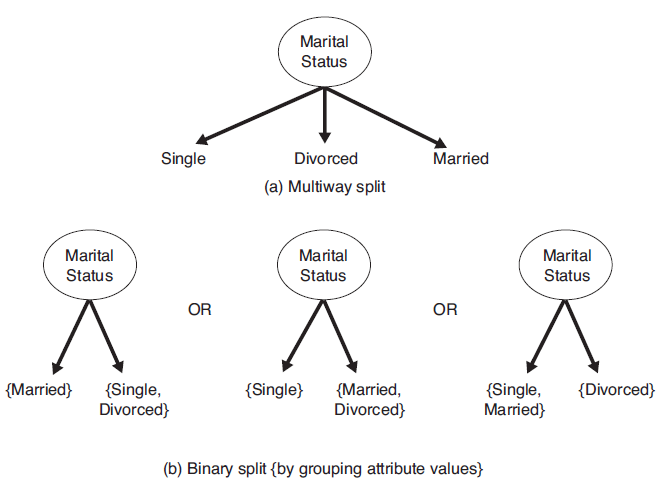
\includegraphics[scale=0.65]{Images/tree_nominal.png}
						\caption{Division d'attributs binaires}
						\label{fig:tree:nominal}
					\end{figure}\noindent
				\end{minipage}\hfill
				\begin{minipage}{0.45\textwidth}
					\begin{figure}[H]
						\centering
						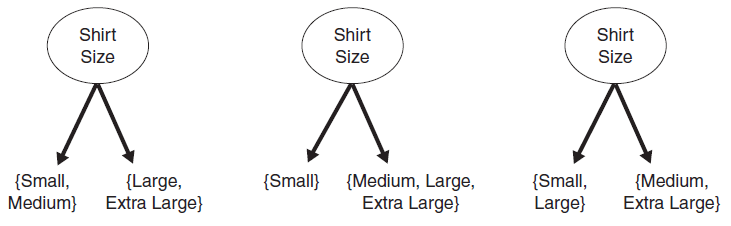
\includegraphics[scale=0.6]{Images/tree_ordinal.png}
						\caption{Division d'attributs ordonnés}
						\label{fig:tree:ordinal}
					\end{figure}\noindent
					\begin{figure}[H]
						\centering
						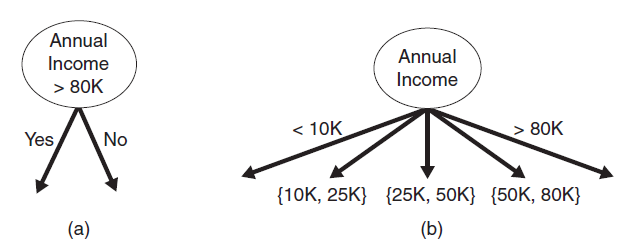
\includegraphics[scale=0.6]{Images/tree_continuous.png}
						\caption{Division d'attributs continus}
						\label{fig:tree:continuous}
					\end{figure}\noindent
				\end{minipage}
				%
			%
			\paragraph{Attributs ordonnés} De la même manière que les 
				nominaux, \hl{tant que l'ordre des attributs n'est pas
				cassé par les partitions}, voir la figure
				\ref{fig:tree:ordinal}.
			%
			\paragraph{Attributs continus} Même chose que les deux derniers,
				même si cette fois, on a une condition sur la valeur
				continue, comme représenté sur la figure
				\ref{fig:tree:continuous}. L'algorithme va
				évaluer les différents splits possibles et choisir le
				meilleur. Pour une division \textit{multiway}, 
				une discrétisation est généralement opérée sur les valeurs
				des attributs.
			%
		%
		\newpage
		%
		\subsection{Qualité d'un partitionnement}\label{sec:tree:split}
			\alinea Pour évaluer la qualité d'un partitionnement, définissons
				$p(i|t)$ comme étant le \textbf{pourcentage} (entre 0 et 1)
				d'objets appartenant à
				la classe $i$, pour un noeud d'arbre $t$. Quand le noeud
				n'est pas utile, la notation peut se réduire à $p_i$.
				Pour une classe binaire, $(p_0, p_1)$ peut-être utilisé
				avec $p_1 = 1 - p_0$.
			%
			\paragraph{\point Impureté d'un noeud}~\\~\\
			%
			\alinea Plus une classe majoritairement représentée par les 
				objets du noeud, au plus ce noeud, cette partition, sera
				considérée comme \textit{pure}. En pratique, c'est le degré
				d'impureté qui sera mesuré. un noeud $(0, 1)$ n'a aucune 
				impureté, tandis qu'un noeud $(0.5, 0.5)$ est le plus impur
				possible (aucune classe n'est majoritairement représentée).\\
			%		
			\alinea Quelques \hl{exemples de mesures d'impuretés} ($c$
				= le nombre de classes différentes, et $0log_20 = 0$
				pour le calcul de l'\textit{Entropy}) :
			\begin{align*}
				\text{Entropy}(t) &= -\sum^{c-1}_{i=0} p(i|t) 
					\cdot log_2 \cdot (p(i|t))\\
				\text{Gini}(t)    &= 1- \sum^{c-1}_{i=0}[p(i|t)]^2\\
				\text{Classification error}(t) &= 1-\max_{i}[p(i|t)]
			\end{align*}
			%
			\alinea Les trois mesures, bien que différentes, respecte
				toutes la mesure "d'impureté" et ont donc le même pire cas
				et le même meilleur cas. Cependant, la mesure choisie peut
				influencer le résultat du partitionnement.
			%
			\paragraph{\point Impureté d'un split}~\\~\\
			% 
				\alinea Pour évaluer 
				l'impureté d'un partitionnement, on va utiliser une
				moyenne pondérée par rapport au nombre d'objet
				par partition.
				$$ I(\text{split}) = \sum_{j=1}^{k}\frac{N(v_j)}{N} 
					I(v_j) $$
				Avec $I$ la mesure d'impureté, $k$ le nombre de partitions,
				$N$ le nombre total d'objets, et $N(v_j)$ le nombre d'objets
				présents dans la partition (noeud fils) $v_j$.
			%
			\begin{figure}[H]
				\centering
				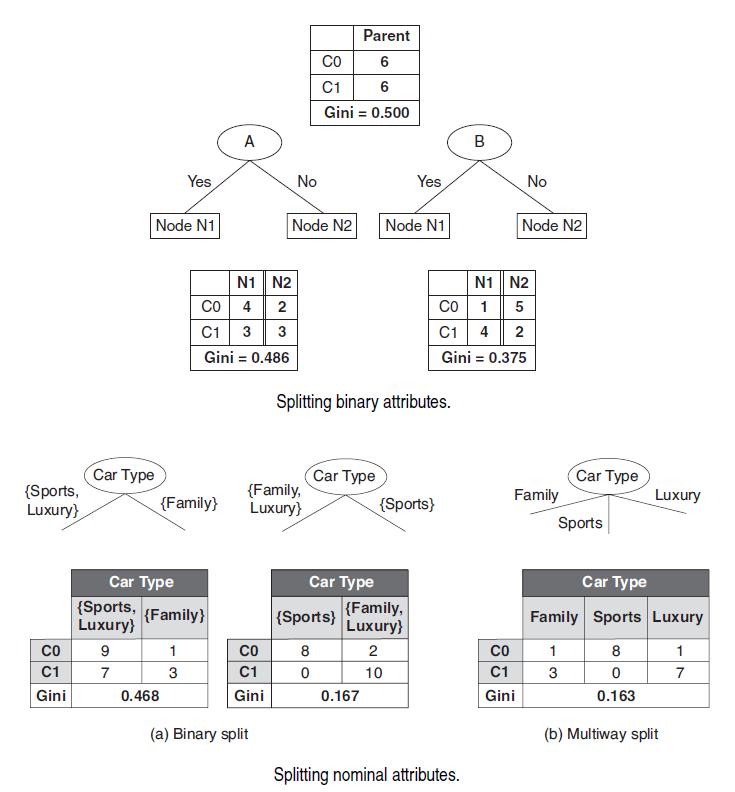
\includegraphics[scale=0.8]{Images/tree_split_measure.png}
				\caption{Exemple de $\text{Gini}(\text{split})$ de
						 partitionnements d'attributs 
						 binaires et nominaux}
				\label{fig:tree:split_measure}
			\end{figure}\noindent
			%
			Par exemple, prenons la figure \ref{fig:tree:split_measure},
			le tableau \texttt{Car Type} ((b), split \textit{multiway}).
			Le calcul se fait comme suit ($\{value\}$ représentant un 
			noeud fils, une partition) : 
			\begin{align*}
				\text{Gini}(\text{split}) &= \frac{4}{20} \cdot 
					\text{Gini}(\{\text{Family}\}) + \frac{8}{20} \cdot 
					\text{Gini}(\{\text{Sports}\}) + \frac{8}{20} \cdot 
					\text{Gini}(\{\text{Luxury}\})\\
				%
				\text{Gini}(\text{split}) &= 
				\frac{4}{20} \cdot 
				[1 - (\sum_{i=0}^{1}[p(C_i|\{\text{Family}\})]^2] + 
				\frac{8}{20} \cdot 
				[1 - (\sum_{i=0}^{1}[p(C_i|\{\text{Sports}\})]^2]\\ 
				&+ 
				\frac{8}{20} \cdot 
				[1 - (\sum_{i=0}^{1}[p(C_i|\{\text{Luxury}\})]^2])\\
				%
				\text{Gini}(\text{split}) &= \frac{4}{20} \cdot 0.375
					 + \frac{8}{20} \cdot 0
					 + \frac{8}{20} \cdot 0.163 = 0.163
			\end{align*}
			C'est normal que le \textit{multiway} ait de meilleurs résultats
				que les binaires, car faire du binaire, c'est en quelques
				sorte fusionner	des résultats de \textit{multiway}\\	
			%
			\begin{figure}[H]
				\centering
				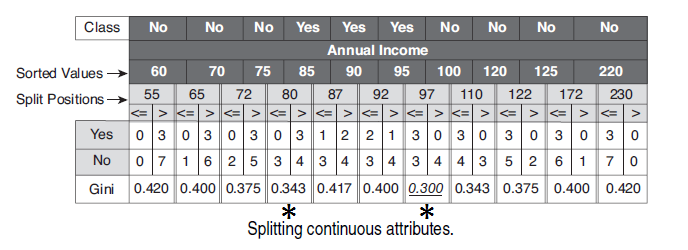
\includegraphics[scale=1.0]{Images/tree_split_measure2.png}
				\caption{Exemple de Gini$($split$)$ d'un partitionnement
						 d'attribut continu}
				\label{fig:tree:split_measure2}
			\end{figure}\noindent
			%
			\alinea En ce qui concerne les attributs continus, 
				il faut réduire 
				le nombre de calculs pour décider du meilleur split. 
				Regardons la figure \ref{fig:tree:split_measure2}.
				\hl{Pour réduire les calculs, on va classer les objets 
				par leur valeur d'attribut
				(Sorted Values). Ensuite, on choisit des positions de split
				en prenant des points à égales distances de deux 
				valeurs ordonnées} (Split Positions, 
				$\lfloor\frac{70 + 75}{2}\rfloor = 72$). \hl{On calcule 
				ensuite
				comme précédemment la valeur de Gini pour chaque split
				 possible},
				et le split en 97 est le meilleur par sa moyenne pondérée 
				d'impureté de 0.300.\\
			%
			\alinea \hl{On pourrait encore améliorer ceci en ne calculant 
				l'impureté que des positions de split se trouvant à la
				frontière de deux classe}. On ne garderait alors que 
				les position marqués par des $\ast$, ce qui réduit 
				considérablement les calculs.
			%			
			\paragraph{\point Gain}~\\~\\
			%
			\alinea Les algorithmes de construction d'arbres choisissent 
				généralement une fonction qui maximise \hl{le gain ($\Delta$)}, 
				c'est-à-dire qui choisisse le partitionnement qui
				améliore le plus la pureté du split comparé à la pureté
				du parent.
				$$ \Delta = I(\text{parent}) - I(\text{split}) $$
			%
			Avec $I$ la mesure d'impureté. Lorsque $I$ 
			correspond à l'\textit{Entropy}, le gain est appelé gain 
			d'information ($\Delta_{\text{info}}$). On remarque que
			\hl{maximiser $\Delta$ revient à minimiser la moyenne pondérée de 
			l'impureté des noeuds fils}.
			%
			\newpage
			%
			\paragraph{\point Ratio de gain}~\\~\\
			%
			\alinea Il peut arriver qu'un attribut soit inapproprié à
				la classification. Typiquement, on retrouve souvent un 
				attribut "ID" dans les tables. Chaque objet ayant un
				ID unique, l'attribut ne peut en aucun cas aider à la
				classification. De manière générale, on voudrait éviter
				qu'un attribut ne divise l'arbre en trop de branches.\\
			%
			\alinea Pour éviter ceci, il y a deux manières de faire :
			\begin{enumerate}
				\item Se restreindre à des splits binaires
				\item Prendre en compte dans le score d'un split le nombre 
					de partitions, comme le fait par exemple le 
					\textbf{Gain ratio}.
			\end{enumerate}
			$$ \text{Gain ratio} = \frac{\Delta_{\text{info}}}%
				{\text{Entropy}(split)}$$
			Ou Entropy$(split)$ est l'impureté du split, calculé avec
				l'\textit{Entropy}. \hl{L'idée est que si le split a 
				beaucoup de branches, alors Entropy$(split)$ sera grand,
				réduisant ainsi son \textit{Gain ratio}.}
			%
		%
		\subsection{Algorithme}
			\begin{figure}[H]
				\centering
				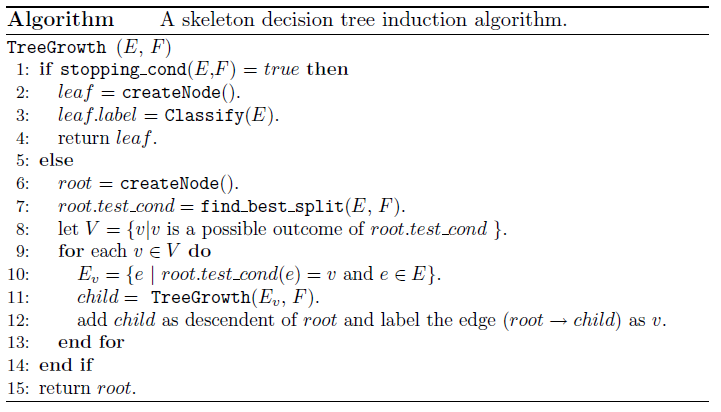
\includegraphics[scale=0.8]{Images/tree_algo.png}
				\caption{}\label{fig:tree:algo}
			\end{figure}\noindent
			%			
			\verb|Classify()| consiste à chercher un label à 
			la feuille. Dans la plupart des cas, cela consiste à faire:
			$$leaf.label = \argmax_{i}{p(i|t)}$$
			\hl{$p(i|t)$ peut dés lors être utilisé comme la probabilité
			qu'à un objet du noeud $t$ d'appartenir à la classe $i$.}\\
			%
			\alinea Après être passé dans l'algorithme, la taille de l'arbre
				peut-être réduite grâce à une étape d'élagage (pruning),
				car les arbres trop larges font souvent l'objet
				d'\textit{overfitting}.
			%
		%
		\subsection{Caractéristiques}
			\alinea Les caractéristiques principales d'une classification
				par arbre de décision sont les suivantes:
			\begin{enumerate}
				\item Technique non-paramétrique. Aucune hypothèse sur le
					jeu de donnée n'est nécessaire.
				\item La recherche de l'arbre optimale $\in NP-Complet$,
					les méthodes utilisées sont des heuristiques.
				\item Les techniques développées sont très rapides 
					d'exécution.
				\item Un arbre est facile à interpréter et à comparer
					à d'autres modèles.
				\item Donne une représentation expressive pour l'apprentissage
					de fonctions à valeurs discrètes. \hl{Même s'il y a
					quelques exceptions avec des problèmes Booléens, comme
					la fonction de parité, dont la valeur est 0
					(\textit{resp.} 1) quand il y a un nombre impair 
					(\textit{resp.} pair) d'attribut Booléen. Il faut
					un arbre complet avec $2^d$ noeud ($d$ = nbre d'attribut
					Booléen) pour avoir un arbre permettant de répondre.}
				\item Les arbres sont robustes au bruit.
				\item Les \textbf{attributs redondants} ne posent pas 
					de problèmes. Un attribut est redondant lorsqu'il y a une
					forte corrélation entre cet attribut et un autre.
					\hl{En pratique, quand l'un des deux attributs redondants
					sera utilisé pour un split, l'autre ne sera pas utilisé.}
					Si l'arbre est trop grand, il se peut qu'il y ait tout
					de même des splits redondant, qui seront coupé à l'élagage.
				\item Si une feuille contient trop peu d'objets, on parle
					de \textbf{fragmentation des données}. On peut l'éviter
					en refusant de split lorsqu'on a plus assez d'objets.
				\item Des sous-arbres peuvent être dupliqué dans l'arbre
					de décision. Ceux-ci seront fusionnés dans l'élagage.
				\item Les frontières, formées par les attributs (cf. figure
					\ref{fig:tree:boundaries}), 
					entre les classes sont rectilignes pour les arbres car
					l'étape de division se fait pour un attribut à la fois,
					ce qui empêche de trouver les relations complexes qu'il
					peut y avoir entre les attributs. Des \textbf{arbres
					de décision obliques} peuvent être utilisés pour 
					résoudre ce problème, ils prennent plus qu'un attribut
					pour diviser leurs attributs, ce qui multiplie les
					calculs... Il existe aussi la \textbf{construction 
					inductive}, qui va créer de nouveaux attributs à partir
					des attributs de base qui sont liés entre eux. \hl{Ceci 
					demande moins de calcul car les relations entre
					attributs se calculent une seule fois.}
				\item Le choix de l'impureté n'a pas beaucoup d'influence
					sur la qualité de l'arbre final. \hl{La stratégie
					d'élagage, par contre, peut l'influencer.}
			\end{enumerate}
			%
			\begin{figure}[H]
				\centering
				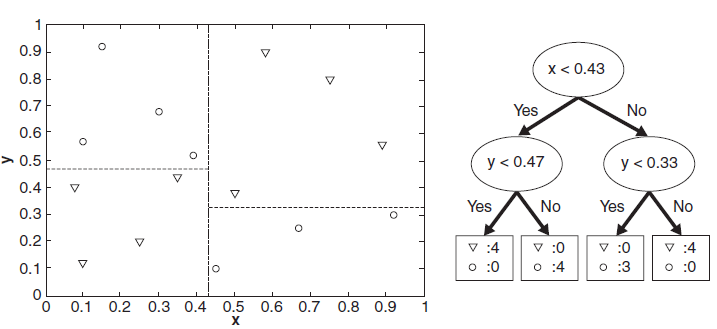
\includegraphics[scale=0.75]{Images/tree_boundaries}
				\caption{Exemple de frontières séparant les classes}
				\label{fig:tree:boundaries}
			\end{figure}\noindent
			%
		%
	%
	\section{Overfitting}
		On divise les erreur de classification en deux types 
			d'erreur : \\
			\begin{enumerate}
				\item \myul{\textbf{\hl{Les erreurs d'entraînement,
				    ou erreurs de resubstitution}}}--
				 \red{Erreurs commises sur les données d'entraînement.}
				\item \myul{\textbf{\hl{Les erreurs de généralisation}}}--
				 \red{Erreurs commises sur des données données extérieures,
					ne venant pas du jeu d'entraînement.}
			\end{enumerate}
		%
		\alinea Dans les deux cas, l'erreur représente le nombre d'objets
			mal classifiés sur le nombre total d'objet du jeu de données.\\
		%
		~\\
		%
		\alinea Un modèle présentant plus d'erreur de généralisation 
			que d'erreur
			d'entraînement est ce qu'on appel un modèle qui fait de
			l'\hl{\textit{overfitting}}, c'est-à-dire qu'il colle trop à ses
			données d'entraînement et qu'il n'est pas très bon pour classer
			d'autres objets, même s'il esst peut-être bon pour les données
			d'entraînement. \\
		%
		\alinea Lorsqu'un modèle est trop restreint, il peut y avoir
			le phénomène d'\textit{\hl{underfitting}} qui apparaît.
			Ceci veut dire que le modèle n'a pas saisi les caractéristiques
			qui permettent de classifier correctement et est donc mauvais
			à la fois pour classer les données d'entraînement, mais aussi
			pour classer les données extérieures.
		%
		\subsection{Bruit}
			\alinea Le bruit est une des causes dee l'\textit{overfitting}.
				Si par exemple des objets sont mal classifiés dans le jeu de 
				données d'entraînement, cela va induire en erreur le modèle
				et peut donc commettre cette erreur en essayant de classifier
				des données extérieures.\\
			%
			\alinea On peut parfois identifier la partie du modèle
				qui pose problème, et la supprimer.
			%
		%
		\subsection{Manque de représentativité}
			\alinea Si il y a un petit nombre d'objets, ou du moins, 
				qu'une classe compte un petit nombre d'objets dans le
				jeu de données d'entraînement, le modèle
				va avoir du mal à identifier ce qui caractérise cette 
				classe mal représentée (e.g. 5 $no$, 1 $yes$).
			%
		%
		\subsection{Procédure de comparaison multiple}
			\alinea Pour illustrer ce qu'est la comparaison multiple,
				imaginons qu'on doive prédire s'il va pleuvoir demain.
				Si on tire au hasard, la probabilité qu'on ait raison
				est de 0.5. Par contre, si on doit prédire pour les 
				dix prochains jour, la probabilité qu'on ait raison
				au moins 8 fois sur 10 est de :
				$$ \frac{\binom{10}{8} + \binom{10}{9} + \binom{10}{10}}%
						{2^{10}} = 0.0547 $$
			%			
			\alinea Ce n'est pas très élevé, mais si on demande à 50
				personnes de faire le même travail pour les 10 jours à venir,
				$Nobody$ étant la probabilité que personne n'ait raison
				au moins pour 8 jours, et $AtLeastOne$ la probabilité qu'au
				moins une des 50 personnes ait raison 8 fois sur 10 :
				$$ Nobody = (1-0.0547)^{50} $$
				$$ AtLeastOne = 1 - Nobody = 0.9399 $$
			%
			\alinea Mais même si l'on trouve la personne qui a trouvé, 
				rien ne garanti que cette même personne est douée dans
				ce qu'elle fait. Peut-être qu'elle a juste deviné au hasard, 
				huit jours de suite.\\
			%
			\alinea On peut faire l'analogie avec la construction d'un arbre
				de décision. Si l'on dit qu'on a un arbre $T_0$ et qu'on
				cherche, parmi $k$ splits différents du noeud courant, 
				$T_{x_{max}}$, l'arbre résultant de l'ajout du split, de
				gain maximum.\hl{ Et si l'on dit que l'on choisit $T_{x_{max}}$
				pour continuer plutôt que $T_0$ si ce gain dépasse un 
				seuil $\alpha$ ($\Delta(T_0, T_{x_{max}}) > \alpha$).
				Et bien plus $k$ augmente, plus on a de chance de trouver 
				le split qui va donner un gain assez élevé}. Mais 
				si le nombre de donnée est réduit, la variance de ce gain
				est plus grand, et il y a de grandes chances qu'un gain
				"hasardeux" soit choisi car il dépassait $\alpha$ (à l'image
				du météorologiste chanceux, on a aucune garantie que cet
				ajout au modèle restera performant pour les données
				extérieures).
			%
		%
		\subsection{Estimation des erreurs de généralisation}
			\alinea La complexité d'un modèle influence l'\textit{overfitting}.
				\hl{La question est donc quelle est la complexité idéale pour
				un modèle ?} Il faudrait minimiser le taux d'erreur de 
				généralisation, mais lors de la création du modèle, 
				l'algorithme n'a accès qu'aux données d'entraînement.
			%
			\subsubsection{Estimation par resubstitution}
			%
			\alinea On suppose ici que le jeu de données d'entraînement
				représente bien les données globales du problème. Il suffit
				donc de minimiser l'erreur d'entraînement pour minimiser,
				par hypothèse, l'erreur de généralisation. 
				\red{Pas bon en pratique.}
			%
			\subsubsection{Incorporation de la complexité du modèle}
			%
			\alinea Comme l'\textit{overfitting} peut venir d'un modèle
				trop complexe, préférer des modèles plus simples permettrait
				de limiter l'\textit{overfitting}, c'est le principe
				du \textbf{Rasoir d'Occam}.\\~\\
				\begin{tabular}{lp{13.5cm}}
					\myul{\textbf{Rasoir d'Occam}}-- & 
						\red{Parmi deux modèles avec la même erreur de 
							 généralisation, le modèle le plus simple des
							 deux est préféré au plus complexe.}
				\end{tabular}~\\~\\
			%
			\alinea Comme disait Einstein, \hl{"Tout devrait être fait le 
				plus simple possible, mais pas plus simple"}. Il ne faudrait
				donc pas prendre un modèle trop simple, au risque 
				d'\textit{underfitting}.\\
			%
			\alinea Ci-dessous sont présenté deux méthodes d'intégration
				de la complexité dans l'évaluation des modèles.
			%
			\paragraph{\point Estimation pessimiste de l'erreur}~\\~\\
				On additionne
				l'erreur d'entraînement et la complexité du modèle. 
				Appelons $n(t)$ le nombre d'objets d'entraînement classifié 
				par le noeud $t$ et $e(t)$ le nombre d'objet mal classifiés.
				l'estimation pessimiste de l'erreur d'un arbre $T$, $e_g(T)$
				est la suivante :
				$$ e_g(T) = \frac{\sum_{i=1}^{k}[e(t_i) + \Omega(t_i)]}%
				                 {\sum_{i=1}^{k}n(t_i)}
				          = \frac{e(T) + \Omega(T)}{N_t} $$
				Avec $k$ le nombre de feuilles, $e(T)$ 
				l'erreur globale d'entraînement, $N_t$ le nombre d'objets
				d'entraînement, et $\Omega(T)$ la pénalité associée à 
				chaque noeud $t_i$. La valeur de cette pénalité décidera
				de l'importance que l'on accorde à la complexité dans 
				l'estimation. \\
				%
				~\\				
				%
				\hl{Pour un arbre binaire, une pénalité de 0.5
				indique qu'un noeud doit toujours se diviser en deux}
				si la division permet de mieux classer au moins un objet 
				d'entraînement, en effet, ajouter une pénalité de 0.5
				à l'erreur en créant une nouvelle feuille 
				(on en crée deux, mais
				on ajoute qu'une seule feuille, étant donné que le parent 
				était précédemment une feuille, et qu'il n'en est plus une)
				est moins couteux que de commettre une erreur d'entraînement.
				\hl{Et une pénalité valant 1 indique que pour diviser un noeud,
				il faut que la division permette d'améliorer 
				la classification d'au moins deux objets d'entraînement.}
				%
			%
			\newpage
			%
			\paragraph{\point Description de longueur minimal (\hl{MDL})}~\\~\\
				Approche venant de la théorie de l'information.
				En prenant la figure \ref{fig:mdl} comme exemple,
				où $A$ et $B$ partage un jeu de donnée $X$, mais où il
				n'y a que $A$ qui connait $y$.
				$A$ voudrait donc transmettre les labels ($y$)
				à $B$, ce qui représente $O(n)$ bits d'information.
				Si $A$ arrive à créer un modèle permettant de déduire
				$y_i$ de $X_i$, alors \hl{si la taille de l'encodage
				du modèle est inférieur à la taille de l'encodage
				des $y$, il est plus intéressant d'envoyer le modèle
				plutôt que $y$ en entier}.\\
				%
				~\\
				%
				Il se peut cependant que le modèle ne permettent pas une
				classification sans faute. Il faudra alors envoyer à $B$
				ces objets, mal classifiés, individuellement.
				$$ Cost(model, data) = enc(model) + enc(misclassified) $$
				\hl{$enc(model)$ étant le coût de l'envoi de l'encodage du
				modèle
				et $enc(misclassified)$ le coût de l'envoi de l'encodage
				des objets mal classifiés par le modèle.
				On devrait donc chercher un modèle qui minimise se coût.}	
				%
				\begin{figure}[H]
					\centering
					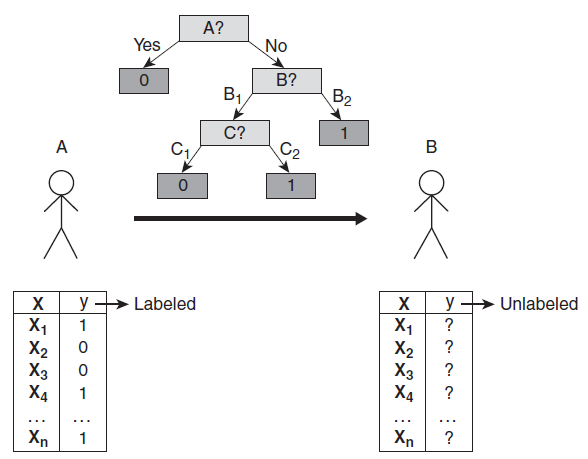
\includegraphics[scale=1.0]{Images/mdl.png}
					\caption{Minimum Description Length (MDL) Principle}
					\label{fig:mdl}
				\end{figure}\noindent
				%
			%
			\newpage
			%
			\subsubsection{Estimer les bornes statistiques}
			%
			\alinea L'erreur de généralisation peut aussi être estimée
				comme une correction statistique de l'erreur d'entraînement.
				On calculera la correction statistique comme une borne
				supérieure de l'erreur d'entraînement, en prenant en compte
				le nombre d'objet qui atteignent une feuille en particulier.
				\hl{Par exemple, l'algorithme \texttt{C4.5} suppose que
				le nombre d'erreurs commises par chaque feuille suit une
				distribution binomiale.} Il faut donc déterminer la borne 
				limite supérieure à l'erreur d'entraînement observée.
			%
			\subsubsection{Utiliser des données de validation}
			%
			\alinea Dans cette méthode, on coupe le jeu de donnée
				d'entraînement en deux. Une partie (généralement $\frac{2}{3})$
				du jeu d'entraînement original est gardé pour l'entraînement
				du modèle et le reste des données est utilisé pour estimer
				l'erreur de généralisation (comme si cette partie des données
				était composée de données extérieures). \red{Le point faible
				de cette méthode est que l'on retire des données du
				jeu d'entraînement, ce qui peut causer des lacunes dans le
				modèle (classe trop peu représentée, ...).}
			%
		%
		\subsection{Overfitting des arbres de décision}
			\alinea \hl{Avoir une estimation fiable de l'erreur 
				de généralisation
				permet à l'algorithme de classification de chercher un 
				modèle précis sans \textit{overfitter} les données d'%
				entraînement.} Ci-dessous sont présentées deux stratégies
				qui permettent d'éviter l'\textit{overfitting} dans les
				arbres de décision.
			%
			\paragraph{\point Prepruning (Early Sotpping Rule)}~\\~\\
			%
			\alinea Le pré-élagage consiste à arrêter la croissance de l'arbre
				avant d'atteindre un arbre qui \textit{overfit} les données
				d'entraînement. Il faut pour cela choisir une \myul{condition
				d'arrêt}. Celle-ci peut se baser sur l'impureté ou le gain.
				La \textbf{principale difficulté} est alors de choisir
				le bon seuil qui arrêtera la croissance de l'arbre pour
				la mesure choisie. Un seuil trop restrictif implique
				de l'\textit{underfitting} et un seuil trop large 
				implique l'\textit{overfitting}.
			%
			\paragraph{\point Post-pruning}~\\~\\
			%
			\alinea On applique le post-élagage sur un arbre qui
				n'a pas subi de \textit{prepruning}. On élague cette fois-ci
				des feuilles vers la racine. Les \hl{deux manière 
				d'élaguer} sont les suivante :
				\begin{enumerate}
					\setlength{\itemsep}{0pt}
					\setlength{\parskip}{0pt}
					\setlength{\parsep}{0pt}
					\item[(1)] \red{Remplacer un sous-arbre par une feuille
						avec le label présent majoritairement dans ce
						sous-arbre.}
					\item[(2)] \red{Remplacer un sous-arbre par se branche 
						la plus utilisée.}
				\end{enumerate}
				L'élagage s'arrête quand il n'y a plus d'améliorations
				possibles.\\
			%
			\alinea On obtient souvent de meilleurs résultats avec le 
				\textit{post-pruning} car on part d'un arbre complet,
				et on évite donc l'\textit{underfitting}. Le point faible 
				pouvant être que les calculs fait pendant la création
				de l'arbre peuvent être "gaspillés" quand on fini par 
				couper une partie de l'arbre.
			%
		%
		\subsection{\'Evaluer les performances d'un classificateur}
			\alinea Maintenant qu'on peut trouver un modèle qui évite
				l'\textit{overfitting}, on va vouloir le tester sur des
				données extérieures, des données de test. \hl{Ceci va 
				permettre d'obtenir une estimation non-biaisée de l'erreur 
				de généralisation} (par la définition de ce type d'erreur).
			%
			\subsubsection{Les métriques}
				\alinea Différentes métriques existent pour évaluer
					les performances d'un modèle sur un jeu de test. 
					Soit $TP$ le nombre de vrai positifs, $TN$ le nombre
					de vrais négatifs, $FP$ le nombre de faux positifs
					et $FN$ le nombre de faux négatifs.
					\begin{align*}
						P &= TP + FN \\
						N &= FP + TN \\~\\
						True-Positive-Rate &= \frac{TP}{P} (=TPR) \\
						False-Positive-Rate &= \frac{FP}{N} (=FPR) \\
						Recall &= \frac{TP}{P} \\
						Precision &= \frac{TP}{TP + FP} \\
						Accuracy &= \frac{TP + TN}{P + N} \\~\\
						F-Measure &= 2 \cdot \frac{Recall \cdot Precision}%
							{Recall + Precision} \\
								  &= \frac{2 \cdot TP}{2 \cdot TP + FP + FN}
					\end{align*}
				%
				~\\
				%
				\alinea Il existe une autre mesure, plus complexe, appelée
					$ROC$. Pour l'expliquer, prenons les figures 
					\ref{fig:roc1} à \ref{fig:roc3}. Le but est d'évaluer
					la capacité d'un attribut (pour l'exemple : $Score$)
					à classer les instances. En effet, certains attributs 
					permettent de mieux distinguer les classes grâce à
					une conditions sur ses valeurs.\\
				%
				~\\
				%
				\alinea En prenant l'exemple de la figure \ref{fig:roc1},
					la valeur la plus haute (au niveau des diagonales),
					est celle de l'instance 6. Au plus cette diagonale
					tend vers le haut-gauche du graphe, au mieux l'attribut
					coupe bien les instances en classes.\\
				%
				\alinea On sait que l'instance 6 est $p$ (le point
					le plus haut est d'office dans la classe testée, ici $p$),
					et que l'instance d'après est $n$ (car sinon, le point
					le plus haut aurait été celui-ci), donc, la condition
					sera :
				%
					$$ \text{Classe } p \text{ si } Score \geq 
						\frac{0.54 + 0.53}{2} \text{; Classe } n 
						\text{ sinon}  $$
					Se faisant, on sait que 0.54 sera de la classe $p$, et que
					0.53 sera dans la class $n$.					
				%
				\begin{figure}[H]
					\centering
					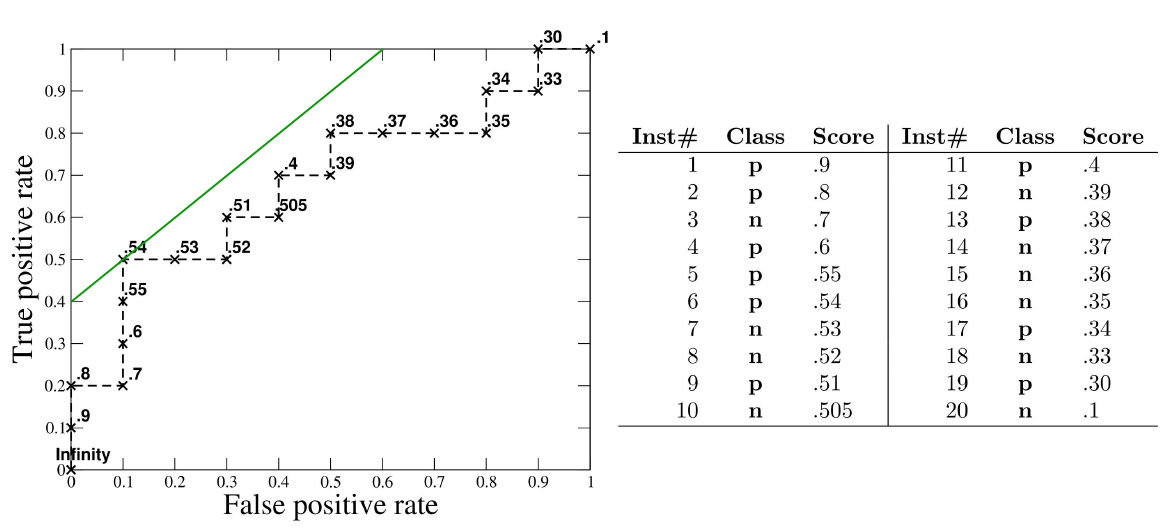
\includegraphics[scale=0.5]{Images/ROC2.png}
					\caption{Pour une instance de $p$, on monte,
							 et pour une instance de $n$, on va à droite}
					\label{fig:roc1}
				\end{figure}\noindent
				\begin{minipage}{0.45\textwidth}
					\vspace*{2cm}
					\begin{figure}[H]
						\centering
						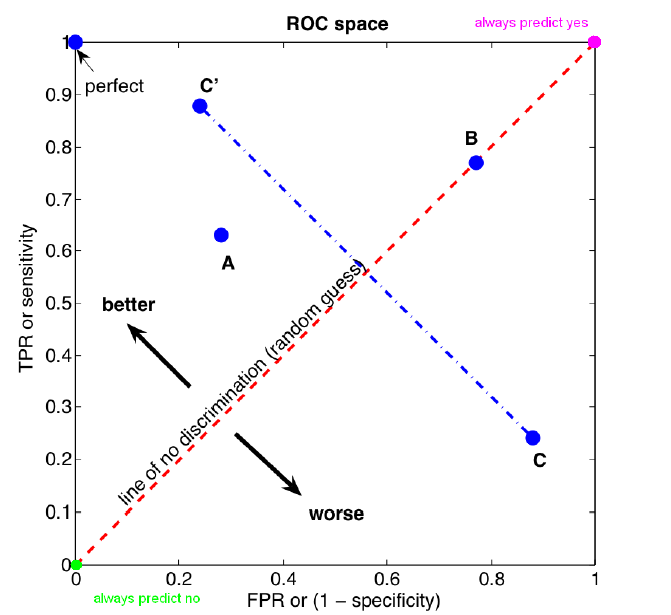
\includegraphics[scale=0.5]{Images/ROC.png}
						\caption{On prend la plus haute diagonale,
								 parallèle à la
								 ligne de discrimination, qui passe
								 par un des points}
						\label{fig:roc2}
					\end{figure}\noindent
				\end{minipage}\hfill
				\begin{minipage}{0.45\textwidth}
					\vspace*{-0.8cm}
					\begin{figure}[H]
						\centering
						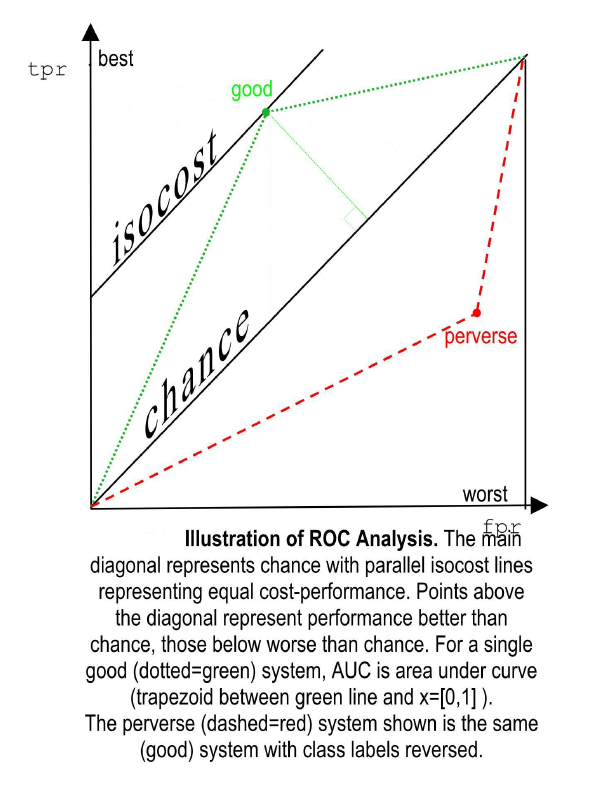
\includegraphics[scale=0.5]{Images/ROC3.png}
						\caption{Au plus la diagonale est haute,
								 au plus la classification est
								 bonne}
						\label{fig:roc3}
					\end{figure}\noindent
				\end{minipage}\noindent
				%
			%
			\subsubsection{Méthode \textit{Holdout}}
				\alinea Très semblable à l'usage de données de validation.
					On va \hl{diviser les données initiales en deux 
					ensembles de même taille. Un des ensemble qui sert 
					de données de test et l'autre de données d'entraînement}.
					\\
				%
				\alinea Les deux ensembles sont donc liés, il peut y avoir 
					un déséquilibre dans les labels. On pourrait donc
					avoir une classe moins représentée dans un ensemble,
					ce qui implique (si les classes sont bien réparties
					dans les données de base) que cette classe est représentée
					trop fort dans l'autre ensemble. Ceci peut impliquer
					un modèle biaisé de par le déséquilibre dans les données
					d'entraînement.
				%
			%
			\subsubsection{Random subsampling}
				\alinea Dans cette méthode, on va répéter la méthode
					\textit{holdout} $k$ fois, la découpe en deux ensemble
					étant aléatoire, chaque découpe sera différente.\\
				%
				\alinea On initialise un compteur $i$. Tant que $i < k$,
					on divise en deux les données, on améliore le modèle et
					on teste le modèle.\\
				%
				\alinea La précision du modèle obtenu est la suivante, 
					avec $acc_i$ la précision du modèle obtenu à 
					l'itération $i$.
					$$ \sum_{i=1}^{k} \frac{acc_i}{k} $$
				%
			%
			\subsubsection{Cross-validation}
				\alinea Cette fois-ci, \hl{chaque objet est utilisé le même
					nombre de fois pour entraîner le modèle, et une 
					seul et unique fois pour le tester.} Cette méthode
					se divise en deux techniques principales.
				%
				\subparagraph{k-fold} On divise les données initiales en
					$k$ sous-ensemble de même taille. \hl{On itère $k$ fois,
					et pour l'itération $i$, on choisit l'ensemble $i$
					comme ensemble de test et les $k-1$ autres comme 
					ensemble d'entraînement.}
				%
				\subparagraph{leave-one-out} Cas particulier du k-fold
					où $k = N$, $N$ étant le nombre d'objets présents dans
					les données. \hl{On a donc un seul objet par 
					sous-ensemble.}
					Cette approche utilise donc $N-1$ données d'entraînement
					à chaque itération (peu de chance d'\textit{underfitting})
					et un seul objet de test (si l'objet ne passe pas le test,
					le modèle sera considéré comme très mauvais). On a donc
					énormément de calculs à faire ($N$ modélisations) mais
					en moyenne le modèle résultant est bon (même si la 
					variance de la qualité du modèle est haute dû aux tests
					à un seul objet).
				%
			%
			\subsubsection{Bootstrap}
				\alinea Contrairement aux méthodes précédentes, les
					objets de cette méthode peuvent être réutilisés
					plusieurs fois pour entraîner le modèle. En effet, 
					la construction d'un extrait de \textit{bootstrap},
					qui sera utilisé comme ensemble d'entraînement se fait
					comme suit :
					\begin{enumerate}
						\setlength{\itemsep}{0pt}
						\setlength{\parskip}{0pt}
						\setlength{\parsep}{0pt}
						\item On tire au hasard un objet et on l'ajoute
							à l'extrait de \textit{bootstrap}.
						\item L'objet tiré est replacé afin qu'il puisse
							peut-être être de nouveau tiré dans une 
							prochaine itération.
						\item Recommencer jusqu'à obtenir un ensemble
							de taille voulue (paramètre).
					\end{enumerate}
					Une fois l'extrait construit, on l'utilise
					comme ensemble d'entraînement, les objets non présents
					dans l'extrait sont utilisés comme données
					de test. On itère $b$ fois, ce qui implique que $b$
					extraits de \textit{bootstrap} sont créés au cours de
					l'opération.\\
				%
				~\\
				%
				\alinea On estime que dans un extrait de taille $N$,
					$N$ étant le nombre d'objet dans le jeu de données de base,
					63,2\% des données de base y sont présent (et donc que
					36,8\% des données sont des doublons).\\
				%
				\alinea La précision d'un modèle construit peut se calculer 
					de plusieurs manières, la plus connue est le
					\textbf{.632 bootstrap}, définie comme suit avec
					$\epsilon_i$ la précision du modèle créé avec 
					l'extrait de \textit{bootstrap} de 
					l'itération $i$, et $acc_s$ la précision d'un modèle
					créé avec tous les objets des données de base en
					entraînement.
					$$ acc_{boot} = \frac{1}{b} \sum_{i=1}^{b}(0.632 
			   					    \cdot \epsilon_i + 0.368 \cdot acc_s) $$
				%
			%
		%
		\subsection{Méthode de comparaison de classificateurs}
		\alinea Pour comparer des résultats de classificateurs,
			surtout sur des jeux de test différents, il faut 
			passer par des tests statistiques. Par exemple,
			prenons deux modèles : $M_a$ et $M_b$. $M_a$ a une 
			meilleure précision que $M_b$, mais la précision de $M_a$
			a été calculé sur un jeu de test moins grand que celui de
			$M_b$. Il faut donc pouvoir mesurer la confiance que l'on
			peut accorder à la précision de $M_a$ par rapport à la
			grandeur de son ensemble de test.\\
		%
		~\\
		%
		\alinea Pour connaître l'intervalle de confiance, 
			il faut déterminer la distribution de probabilité
			qui domine la mesure de précision. Pour ce faire,
			on peut modéliser le problème de classification en
			une expérience binomiale:
			\begin{enumerate}
				\setlength{\itemsep}{0pt}
				\setlength{\parskip}{0pt}
				\setlength{\parsep}{0pt}
				\item Expérience de $N$ essais indépendants 
					donnant soit un \myul{succès}, 
					soit un \myul{échec}.
				\item La probabilité $p$ d'obtenir un succès à chaque
					essai est constante.
			\end{enumerate}
		%
		\newpage
		%
			Soit $X$ le nombre de succès sur $N$ essais, la 
			probabilité d'en avoir $v$ est la suivante:
			$$ P(X=v) = \binom{N}{v} p^v (1 - p)^{N-v} $$
		%				
		\alinea \hl{Pour la classification, $p$ est la vrai précision
			du modèle, $X$ est le nombre d'instances bien classifiées,
			$N$ le nombre total d'objets.} Si on prends la précision
			empirique, normalisée par rapport à la taille du jeu
			de données de test, \hl{$\frac{X}{N}$} (moyenne = $p$, 
			variance = $\frac{p(1 - p)}{N}$), c'est aussi une 
			distribution normale. Son intervalle de confiance est
			souvent approximé par une distribution normale pour
			$N$ suffisamment grand : 
			$$ P \left( -Z_{\alpha/2} \leq \frac{acc - p}%
				{\sqrt{p(i-p)/N}} \leq Z_{1-\alpha/2} \right) 
						= 1 - \alpha $$
			Avec $-Z_{\alpha/2}$ et $Z_{1-\alpha/2}$ les bords
			supérieurs et inférieurs
			obtenus par distribution normale avec une confiance de 
			$1-\alpha$.\\
		%
		~\\
		%
		\alinea Les formules suivantes permettent alors de conclure
			sur la différence entre les précisions comparées/
			$$ I (= d_t) = d \pm z_{\alpha/2} \cdot 
				\hat{\sigma} = \mathbf{[} d - z_{\alpha/2} \cdot 
				\hat{\sigma}\mathbf{,}\ \ d + z_{\alpha/2} \cdot 
				\hat{\sigma}\mathbf{]} $$
			$$ d = e - f $$
			$$ 1-\alpha = 90\%\ (Certitude) \Leftrightarrow 
				\alpha = 10\% $$
			$$ z_{\alpha/2} = 1.65\ (Confiance) $$
			$$ \hat{\sigma} = \sqrt{\dfrac{e(1 - e)}{n} + 
				\dfrac{f(1 - f)}{m}} $$
			Avec $e$ (\textit{resp.} $f$) représente le 
			pourcentage d'instances mal classifiées
			dans le modèle 1 (\textit{resp.} 2) et $n$ 
			(\textit{resp.} $m$) représente le nombre total
			d'instances classées par le modèle 1 (\textit{resp.} 2).\\
		%
		\alinea Les précisions des deux modèles sont alors 
			considérées comme significativement différentes si
			0 n'est pas couvert par I. \\
			%
		%
		~\\
		%
		\myul{\textbf{\hl{Remarque}}} -- On peut aussi utilise l'intervalle
			de confiance pour évaluer un élagage d'arbre. Comme le montre
			la figure \ref{fig:pruning}. On y voit qu'on regarde à élaguer
			le noeud qui a été divisé selon l'attribut "health plan
			contribution". On calcule alors l'intervalle de confiance 
			pour chacun des fils de ce noeud, en prenant en compte la 
			précision du fils concernant la classe "bad".\\
			On a donc $n$ le nombre d'objet total, $X$ le nombre d'objet
			libellé "bad", et $p_1$ et $p_2$ les bornes, inférieure et 
			supérieures, de l'intervalle de confiance.
		%
		\begin{figure}[H]
			\centering
			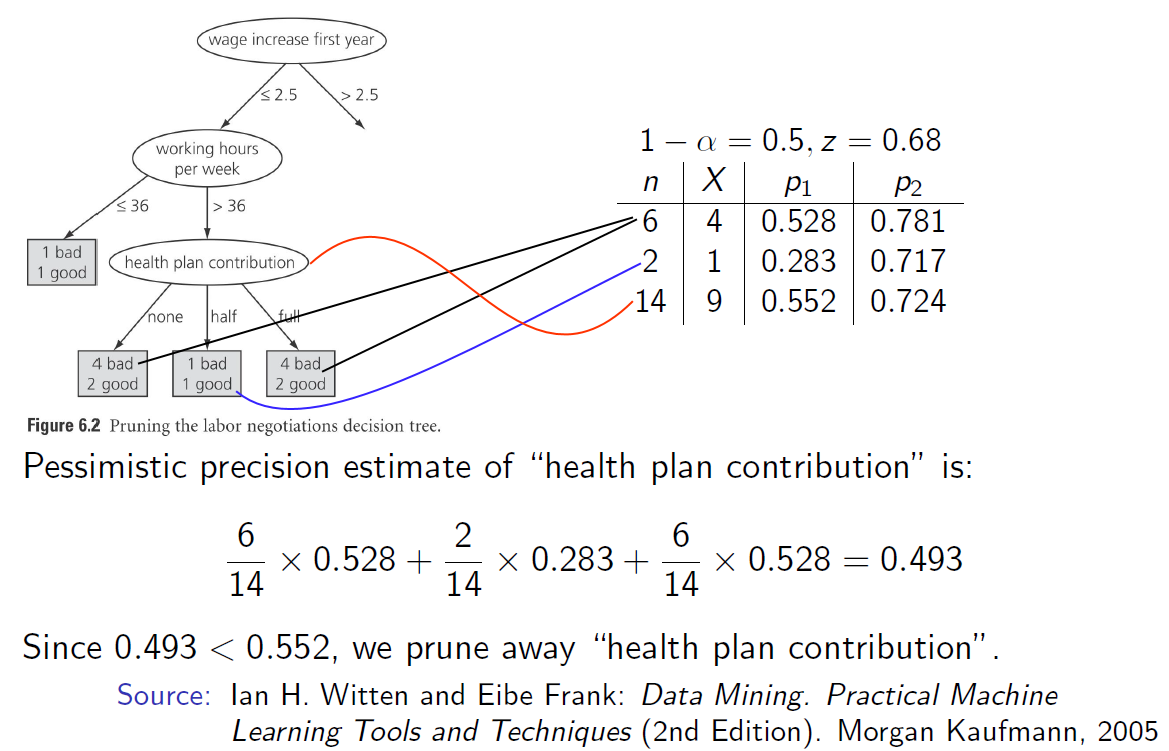
\includegraphics[scale=0.45]{Images/pruning.png}
			\caption{L'élagage est dans ce cas utile devrait être fait,}
					 car le split n'apporte pas d'informations utiles.
			\label{fig:pruning}
		\end{figure}\noindent
		%
		\alinea On compare donc ensuite la somme pondérée de la borne 
			inférieure des fils (estimation \myul{pessimiste}) avec
			la borne inférieur du parent. Si cette dernière est 
			plus élevée (comme dans l'exemple), cela veut dire que
			la division n'était pas utile et fait perdre en confiance, 
			on peut donc élaguer.
		%
	%
	\newpage
	%
	\section{Types d'algorithmes}
		\alinea Il existe plusieurs type d'algorithmes construisant des 
			modèles de classification. En voici quelques-uns.
		%
		\subsection{Nearest Neighbours (IBk, Lazy)}
			\alinea Cette technique s'appuie sur la notion de distance
				entre les instances. Plusieurs distances peuvent être
				considérées (Euclidienne, Manhattan, ...). Voici quelques
				définitions de \hl{distances} en fonction des 
				types d'attributs.
				\begin{itemize}
					\setlength{\itemsep}{0pt}
					\setlength{\parskip}{0pt}
					\setlength{\parsep}{0pt}
					\item \myul{Un attribut numérique uniquement} : différence.
					\item \myul{Plusieurs attributs numériques} : normalisation
						des valeurs + distance Euclidienne, ou Manhattan.
					\item \myul{Attributs nominaux} : 0 si valeur identique,
						1 sinon.
				\end{itemize}
			%
			\alinea Il reste ensuite à regrouper les objets en groupe en 
				fonction de la distance qu'il y a entre chaque objets
				et leur $k$ plus proches voisins.
			%
		%
		\subsection{Règles de classification}
			\alinea Classificateur qui consiste en une série de $k$ 
				règles, liées entre-elles par des "ET".\\				
			%
			\alinea Exemple :
				\begin{center}
					Si $a < 5$ et $b < 4$ : classe = oui\\
					Si $a > 2$ et $c > 3$ : classe = non\\
					Si $b > 3$ et $d > 2$ : classe = oui\\
					...
				\end{center}
			%
			\alinea Pour le classificateur \hl{\texttt{OneR}}, le but est
				de tester pleins de règles concernant chacune un seul
				attribut, chaque règle testées prenant les meilleurs
				valeurs "limites" de l'attribut pour classifier, et seule
				la meilleure règle est gardée.\\
			%
			~\\
			%
			\alinea Pour \hl{\texttt{Prism}} par contre, on se concentre 
				sur les classes. Prenons comme exemple la figure 
				\ref{fig:prism} comme exemple. Dans cet exemple, il y 
				a deux classes : "oui", et "non", avec 5 objets dans 
				chaque classe. On va ici s'intéresser 
				à classer "non" au mieux. On va donc énumérer des
				règles simples (cf. figure \ref{fig:prism}), et 
				regarder la précision de classification des instances
				correspondant à ces conditions.
			%
			\begin{figure}[H]
				\centering
				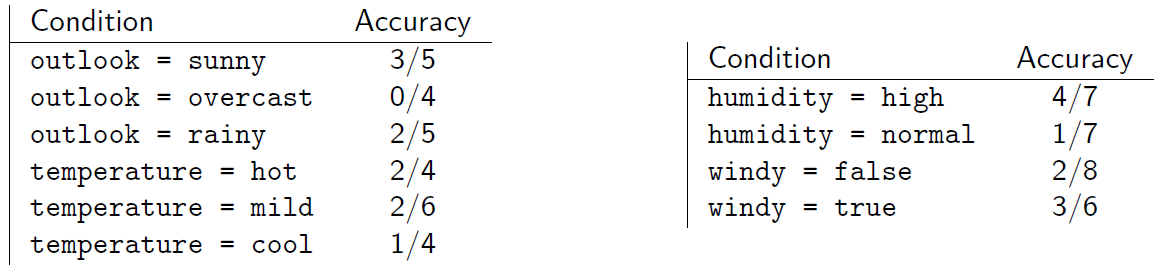
\includegraphics[scale=1.0]{Images/prism.png}
				\caption{Règle et précision de classification pour la classe
						 "non"}
				\label{fig:prism}
			\end{figure}\noindent
			%
			\alinea La précision la plus élevée est 3/5. Nous choisissons
				donc la condition \texttt{outlook = sunny}. On va ensuite 
				regarder s'il faut continuer à chercher des règles ou pas.
				La figure \ref{fig:prism2} montre les 5 instances
				correspondant à la condition \texttt{outlook = sunny}
				que l'on vient de choisir.
			%
			\begin{figure}[H]
				\centering
				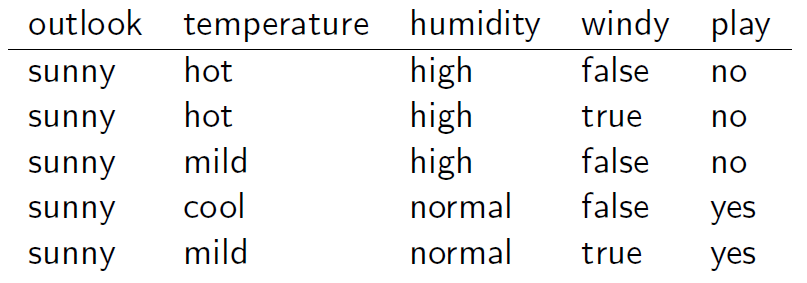
\includegraphics[scale=1.0]{Images/prism2.png}
				\caption{On peut encore raffiner la condition en
						 rajouter des conditions}
				\label{fig:prism2}
			\end{figure}\noindent
			%
			\alinea Si on recommence à regarder pour quelle règle 
				on classe le mieux les "non" pour les cinq instances
				restantes, on obtient le tableau de la figure \ref{fig:prism3}.
			%
			\begin{figure}[H]
				\centering
				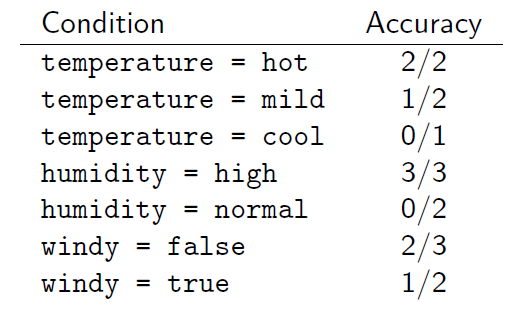
\includegraphics[scale=1.0]{Images/prism3.png}
				\caption{L'égalité entre deux règles se brise par le
						 le nombre d'instances couvertes}
				\label{fig:prism3}
			\end{figure}\noindent
			\alinea On remarque une égalité entre \texttt{temperature = hot}
				et \texttt{humidity = high}. Nous prendrons la deuxième 
				condition car c'est elle des deux qui couvre le plus d'objets.
				Seulement, la règle entière \texttt{si outlook = sunny et
				humidity = high} ne couvre que 3 ces 5 instances "non".
				On recommence depuis le début, mais cette fois-ci en
				retirant les objets répondant à la règle déjà trouvée,
				etc... jusqu'à obtenir le maximum d'instances "non" bien 
				classées. Puis, on peut recommencer le travail avec les
				classes "yes".\\
			%
			~\\
			%
			\myul{\hl{\textbf{Remarque}}} -- Les règles trouvées par
				\texttt{Prism} sont \textit{sound} mais pas 
				\textit{complete}. En effet, on est sur que \myul{les 
				règles sont vraies pour le jeu de données} d'entraînement
				(\textit{sound}) mais elles ne sont \myul{pas vraies pour 
				n'importe quel jeu de données} (non \textit{complete})
			%
		%
		\newpage
		%
		\subsection{Arbres IBk}
			\alinea Arbres de décisions avec des règles sur les attributs.
				On peut noter que ces arbres sont parfois trop complexes
				pour rien (problème du sous arbres dupliqué), et que 
				les règles s'y trouvant ne sont pas garantie \textit{sound}
				ni \textit{complete}. \\
			%
			~\\
			%
			\alinea On peut noter qu'il y a deux types de règles de manière 
				générale (pas que pour les arbres). Ceux-ci sont expliqués
				sur la figure \ref{fig:ibk}.
			%
			\begin{figure}[H]
				\centering
				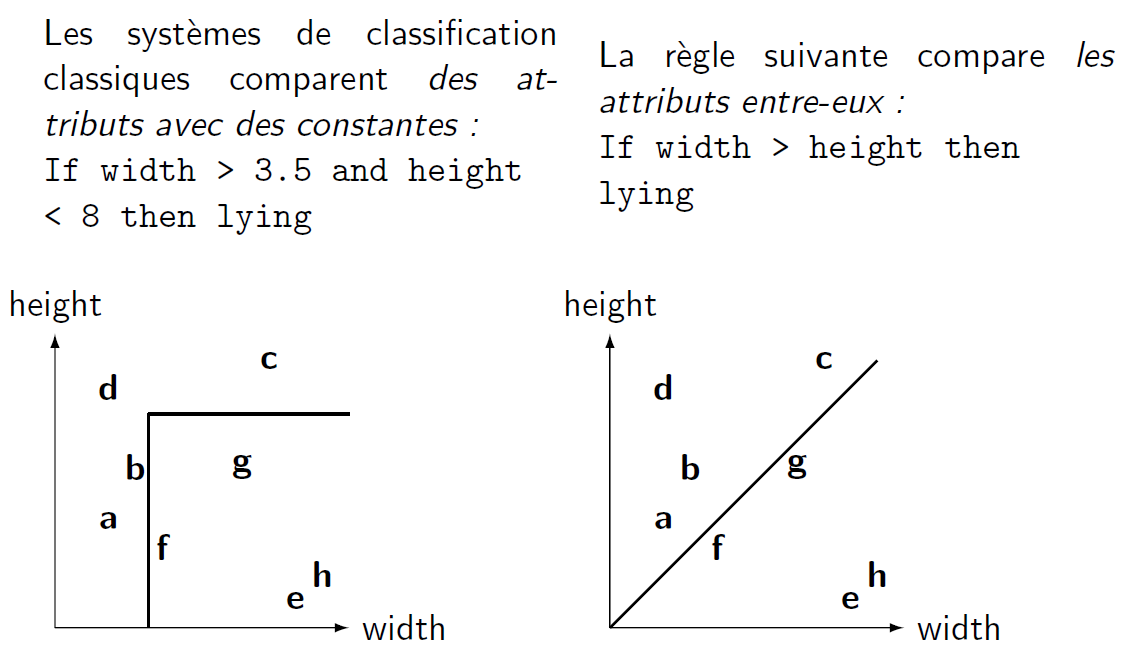
\includegraphics[scale=0.3]{Images/ibk.png}
				\caption{Il y a deux types de règles}
				\label{fig:ibk}
			\end{figure}\noindent
			%
		%
		\subsection{Naive Bayes}
			\alinea	Ce classificateur utilise la règle de Bayes. C'est une 
				règle de probabilité qui dit : 
				$$ Pr(H | E) = \frac{Pr(E | H) \cdot Pr(H)}{Pr(E)} $$
				Avec $Pr(x | y)$ voulant dire la probabilité de $x$, sachant
				que $y$.\\
			%
			~\\
			%
			\alinea Pour classifier, on utilisera cette règle afin de 
				trouver la probabilité pour l'objet $k$ 
				d'appartenir à une classe $i$, en
				sachant les attributs de cet objet 
				(=$\text{Pr}(Class_i | Attributes_k)$). Normalement, 
				un tel calcul
				est très couteux et parfois infaisable quand on a pas
				toutes les informations, car :
				$$ \text{Pr}(Class_i | Attributes_k) = 
				    \frac{\text{Pr}(Att_{1_k}\& 
					Att_{2_k} \& \ldots \& Att_{j_k}| Class_i) 
					\cdot \text{Pr}(Class_i)}{\text{Pr}(Attributes_k)} $$
				Mais on admet une certaine naïveté, en pensant que tous
				les attributs sont indépendants l'un de l'autre, et donc
				que :
				$$ \text{Pr}(Class_i | Attributes_k) =  \frac{
						\text{Pr}(Att_{1_k} | Class_i) \cdot
						\text{Pr}(Att_{2_k} | Class_i) \cdot
						\ldots \cdot
						\text{Pr}(Att_{j_k} | Class_i) \cdot
						\text{Pr}(Class_i)}{\text{Pr}(Attributes_k)}$$
				Avec $Att_{l_k}$ l'attribut $l$ de l'objet $k$.	
			%
		%
	%
%
\part{Analyse par association}
%
\part{Analyse par clustering}
%
\end{document}